\upaper{41}{Physical Aspects of the Local Universe}
\uminitoc{The Nebadon Power Centres}
\uminitoc{The Satania Physical Controllers}
\uminitoc{Our Starry Associates}
\uminitoc{Sun Density}
\uminitoc{Solar Radiation}
\uminitoc{Calcium --- The Wanderer of Space}
\uminitoc{Sources of Solar Energy}
\uminitoc{Solar-Energy Reactions}
\uminitoc{Sun Stability}
\uminitoc{Origin of Inhabited Worlds}
\author{Archangel}
\vs p041 0:1 The characteristic space phenomenon which sets off each local creation from all others is the presence of the Creative Spirit. All Nebadon is certainly pervaded by the space presence of the Divine Minister of Salvington, and such presence just as certainly terminates at the outer borders of our local universe. That which is pervaded by our local universe Mother Spirit \bibemph{is} Nebadon; that which extends beyond her space presence is outside Nebadon, being the extra\hyp{}Nebadon space regions of the superuniverse of Orvonton --- other local universes.
\vs p041 0:2 \pc While the administrative organization of the grand universe discloses a clear\hyp{}cut division between the governments of the central, super-, and local universes, and while these divisions are astronomically paralleled in the space separation of Havona and the 7 superuniverses, no such clear lines of physical demarcation set off the local creations. Even the major and minor sectors of Orvonton are (to us) clearly distinguishable, but it is not so easy to identify the physical boundaries of the local universes. This is because these local creations are administratively organized in accordance with certain \bibemph{creative} principles governing the segmentation of the total energy charge of a superuniverse, whereas their physical components, the spheres of space --- suns, dark islands, planets, etc. --- take origin primarily from nebulae, and these make their astronomical appearance in accordance with certain \bibemph{precreative} (transcendental) plans of the Architects of the Master Universe.
\vs p041 0:3 One or more --- even many --- such nebulae may be encompassed within the domain of a single local universe even as Nebadon was physically assembled out of the stellar and planetary progeny of Andronover and other nebulae. The spheres of Nebadon are of diverse nebular ancestry, but they all had a certain minimum commonness of space motion which was so adjusted by the intelligent efforts of the power directors as to produce our present aggregation of space bodies, which travel along together as a contiguous unit over the orbits of the superuniverse.
\vs p041 0:4 Such is the constitution of the local star cloud of Nebadon, which today swings in an increasingly settled orbit about the Sagittarius centre of that minor sector of Orvonton to which our local creation belongs.
\usection{The Nebadon Power Centres}
\vs p041 1:1 The spiral and other nebulae, the mother wheels of the spheres of space, are initiated by Paradise force organizers; and following nebular evolution of gravity response, they are superseded in superuniverse function by the power centres and physical controllers, who thereupon assume full responsibility for directing the physical evolution of the ensuing generations of stellar and planetary offspring. This physical supervision of the Nebadon preuniverse was, upon the arrival of our Creator Son, immediately co\hyp{}ordinated with his plan for universe organization. Within the domain of this Paradise Son of God,\fnst{In 1995 text no comma after ``God''.} the Supreme Power Centres and the Master Physical Controllers collaborated with the later appearing Morontia Power Supervisors and others to produce that vast complex of communication lines, energy circuits, and power lanes which firmly bind the manifold space bodies of Nebadon into one integrated administrative unit.
\vs p041 1:2 100 Supreme Power Centres of the fourth order are permanently assigned to our local universe. These beings receive the incoming lines of power from the third\hyp{}order centres of Uversa and relay the down\hyp{}stepped and modified circuits to the power centres of our constellations and systems. These power centres, in association, function to produce the living system of control and equalization which operates to maintain the balance and distribution of otherwise fluctuating and variable energies. Power centres are not, however, concerned with transient and local energy upheavals, such as sun spots and system electric disturbances; light and electricity are not the basic energies of space; they are secondary and subsidiary manifestations.
\vs p041 1:3 The 100 local universe centres are stationed on Salvington, where they function at the exact energy centre of that sphere. Architectural spheres, such as Salvington, Edentia, and Jerusem, are lighted, heated, and energized by methods which make them quite independent of the suns of space. These spheres were constructed --- made to order --- by the power centres and physical controllers and were designed to exert a powerful influence over energy distribution. Basing their activities on such focal points of energy control, the power centres, by their living presences, directionize and channelize the physical energies of space. And these energy circuits are basic to all physical\hyp{}material and morontia\hyp{}spiritual phenomena.
\vs p041 1:4 10 Supreme Power Centres of the fifth order are assigned to each of Nebadon’s primary subdivisions, the 100 constellations. In Norlatiadek, your constellation, they are not stationed on the headquarters sphere but are situated at the centre of the enormous stellar system which constitutes the physical core of the constellation. On Edentia there are 10 associated mechanical controllers and 10 frandalanks who are in perfect and constant liaison with the near\hyp{}by power centres.
\vs p041 1:5 One Supreme Power Centre of the sixth order is stationed at the exact gravity focus of each local system. In the system of Satania the assigned power centre occupies a dark island of space located at the astronomic centre of the system. Many of these dark islands are vast dynamos which mobilize and directionize certain space\hyp{}energies, and these natural circumstances are effectively utilized by the Satania Power Centre, whose living mass functions as a liaison with the higher centres, directing the streams of more materialized power to the Master Physical Controllers on the evolutionary planets of space.
\usection{The Satania Physical Controllers}
\vs p041 2:1 While the Master Physical Controllers serve with the power centres throughout the grand universe, their functions in a local system, such as Satania, are more easy of comprehension. Satania is one of 100 local systems which make up the administrative organization of the constellation of Norlatiadek, having as immediate neighbours the systems of Sandmatia, Assuntia, Porogia, Sortoria, Rantulia, and Glantonia. The Norlatiadek systems differ in many respects, but all are evolutionary and progressive, very much like Satania.
\vs p041 2:2 Satania itself is composed of over 7,000 astronomical\tunemarkup{pgnexus10}{\linebreak} groups, or physical systems, few of which had an origin similar to that of your solar system. The astronomic centre of Satania is an enormous dark island of space which, with its attendant spheres, is situated not far from the headquarters of the system government.
\vs p041 2:3 \pc Except for the presence of the assigned power centre, the supervision of the entire physical\hyp{}energy system of Satania is centred on Jerusem. A Master Physical Controller, stationed on this headquarters sphere, works in co\hyp{}ordination with the system power centre, serving as liaison chief of the power inspectors headquartered on Jerusem and functioning throughout the local system.
\vs p041 2:4 The circuitizing and channelizing of energy is supervised by the 500,000 living and intelligent energy manipulators scattered throughout Satania. Through the action of such physical controllers the supervising power centres are in complete and perfect control of a majority of the basic energies of space, including the emanations of highly heated orbs and the dark energy\hyp{}charged spheres. This group of living entities can mobilize, transform, transmute, manipulate, and transmit nearly all of the physical energies of organized space.
\vs p041 2:5 Life has inherent capacity for the mobilization and transmutation of universal energy. You are familiar with the action of vegetable life in transforming the material energy of light into the varied manifestations of the vegetable kingdom. You also know something of the method whereby this vegetative energy can be converted into the phenomena of animal activities, but you know practically nothing of the technique of the power directors and the physical controllers, who are endowed with ability to mobilize, transform, directionize, and concentrate the manifold energies of space.
\vs p041 2:6 \pc These beings of the energy realms do not directly concern themselves with energy as a component factor of living creatures, not even with the domain of physiological chemistry. They are sometimes concerned with the physical preliminaries of life, with the elaboration of those energy systems which may serve as the physical vehicles for the living energies of elementary material organisms. In a way the physical controllers are related to the preliving manifestations of material energy as the adjutant mind\hyp{}spirits are concerned with the prespiritual functions of material mind.
\vs p041 2:7 \pc These intelligent creatures of power control and energy direction must adjust their technique on each sphere in accordance with the physical constitution and architecture of that planet. They unfailingly utilize the calculations and deductions of their respective staffs of physicists and other technical advisers regarding the local influence of highly heated suns and other types of supercharged stars. Even the enormous cold and dark giants of space and the swarming clouds of star dust must be reckoned with; all of these material things are concerned in the practical problems of energy manipulation.
\vs p041 2:8 The power\hyp{}energy supervision of the evolutionary inhabited worlds is the responsibility of the Master Physical Controllers, but these beings are not responsible for all energy misbehaviour on Urantia. There are a number of reasons for such disturbances, some of which are beyond the domain and control of the physical custodians. Urantia is in the lines of tremendous energies, a small planet in the circuit of enormous masses, and the local controllers sometimes employ enormous numbers of their order in an effort to equalize these lines of energy. They do fairly well with regard to the physical circuits of Satania but have trouble insulating against the powerful Norlatiadek currents.
\usection{Our Starry Associates}
\vs p041 3:1 There are upward of 2,000 brilliant suns\fnst{A sphere centred on Urantia with the radius of 65\,ly contains about 2,000 stars. Therefore, assuming that the star density in other parts of Satania is at least as great as in the vicinity of our Sun, we can deduce that the size of Satania cannot be greater than 65\,ly.} pouring forth light and energy in Satania, and your own sun is an average blazing orb. Of the 30 suns nearest yours, only 3 are brighter\fnst{The 30 nearest stars lie in a sphere of radius 12.6\,ly and the three stars brighter than ours are: $\alpha$ Centauri (4.35\,ly), Sirius (8.57\,ly) and Procyon (11.4\,ly). These are the same three stars mentioned in the source text \cite{Jeans1}.}. The Universe Power Directors initiate the specialized currents of energy which play between the individual stars and their respective systems. These solar furnaces, together with the dark giants of space, serve the power centres and physical controllers as way stations for the effective concentrating and directionizing of the energy circuits of the material creations.
\vs p041 3:2 The suns of Nebadon are not unlike those of other universes. The material composition of all suns, dark islands, planets, and satellites, even meteors, is quite identical. These suns have an average diameter of about $1.6\times 10^6$\,km, that of your own solar orb being slightly less\fnst{Our own ``solar orb'' has an average diameter of $1.392684 \times 10^6$\,km.}. The largest star in the universe, the stellar cloud Antares, has a diameter 680 that of your sun\fnst{According to https://arxiv.org/abs/1304.4800} --- or about a billion kilometres. One could pack about 207 million\fnst{Calculated with the same packing efficiency of 65.8\% for identical spheres that is used in the human source text of \cite{Jeans1}, p.\,183.} of your own suns inside it, and there would still be room to spare. But there is abundant space to accommodate all of these enormous suns. They have just as much comparative elbow room in space as one dozen oranges\fnst{In the human original we have ``thirty cricket balls'' instead.} would have if they were circulating about throughout the interior of Urantia, and were the planet a hollow globe.
\vs p041 3:3 \pc When suns that are too large are thrown off a nebular mother wheel, they soon break up or form double stars. All suns are originally truly gaseous, though they may later transiently exist in a semiliquid state. When your sun attained this quasi\hyp{}liquid state of supergas\fnst{Defined at \bibref[41:4.3]{p041 4:3} as alsmost fully ionized plasma.} pressure, it was not sufficiently large to split equatorially, this being one type of double star formation.
\vs p041 3:4 When less than \bibfrac{1}{10}\ts{th} the size of your sun, these fiery spheres rapidly contract, condense, and cool. When upwards of 30 times its size --- rather 30 times the gross content of actual material --- suns readily split into two separate bodies, either becoming the centres of new systems or else remaining in each other’s gravity grasp and revolving about a common centre as one type of double star.
\vs p041 3:5 \pc The most recent of the major cosmic eruptions in Orvonton was the extraordinary double star explosion, the light of which reached Urantia in A.D.\,1572.\fnst{The supernova SN\,1572 appeared in early November 1572 is known as ``Tycho's supernova'', because in 1573 Tycho Brahe published both his own observations and the analysis of sightings of others. In England, Queen Elizabeth summoned Thomas Allen the mathematician to have his advice about the new Star that appeared in the Cassiopeia. In China, the star was interpreted as an evil omen for the young Wanli Emperor, which, however did not prevent him reigning for the next 48 years.} This conflagration was so intense that the explosion was clearly visible in broad daylight.\tunemarkup{pictures}{\begin{figure}[H]\centering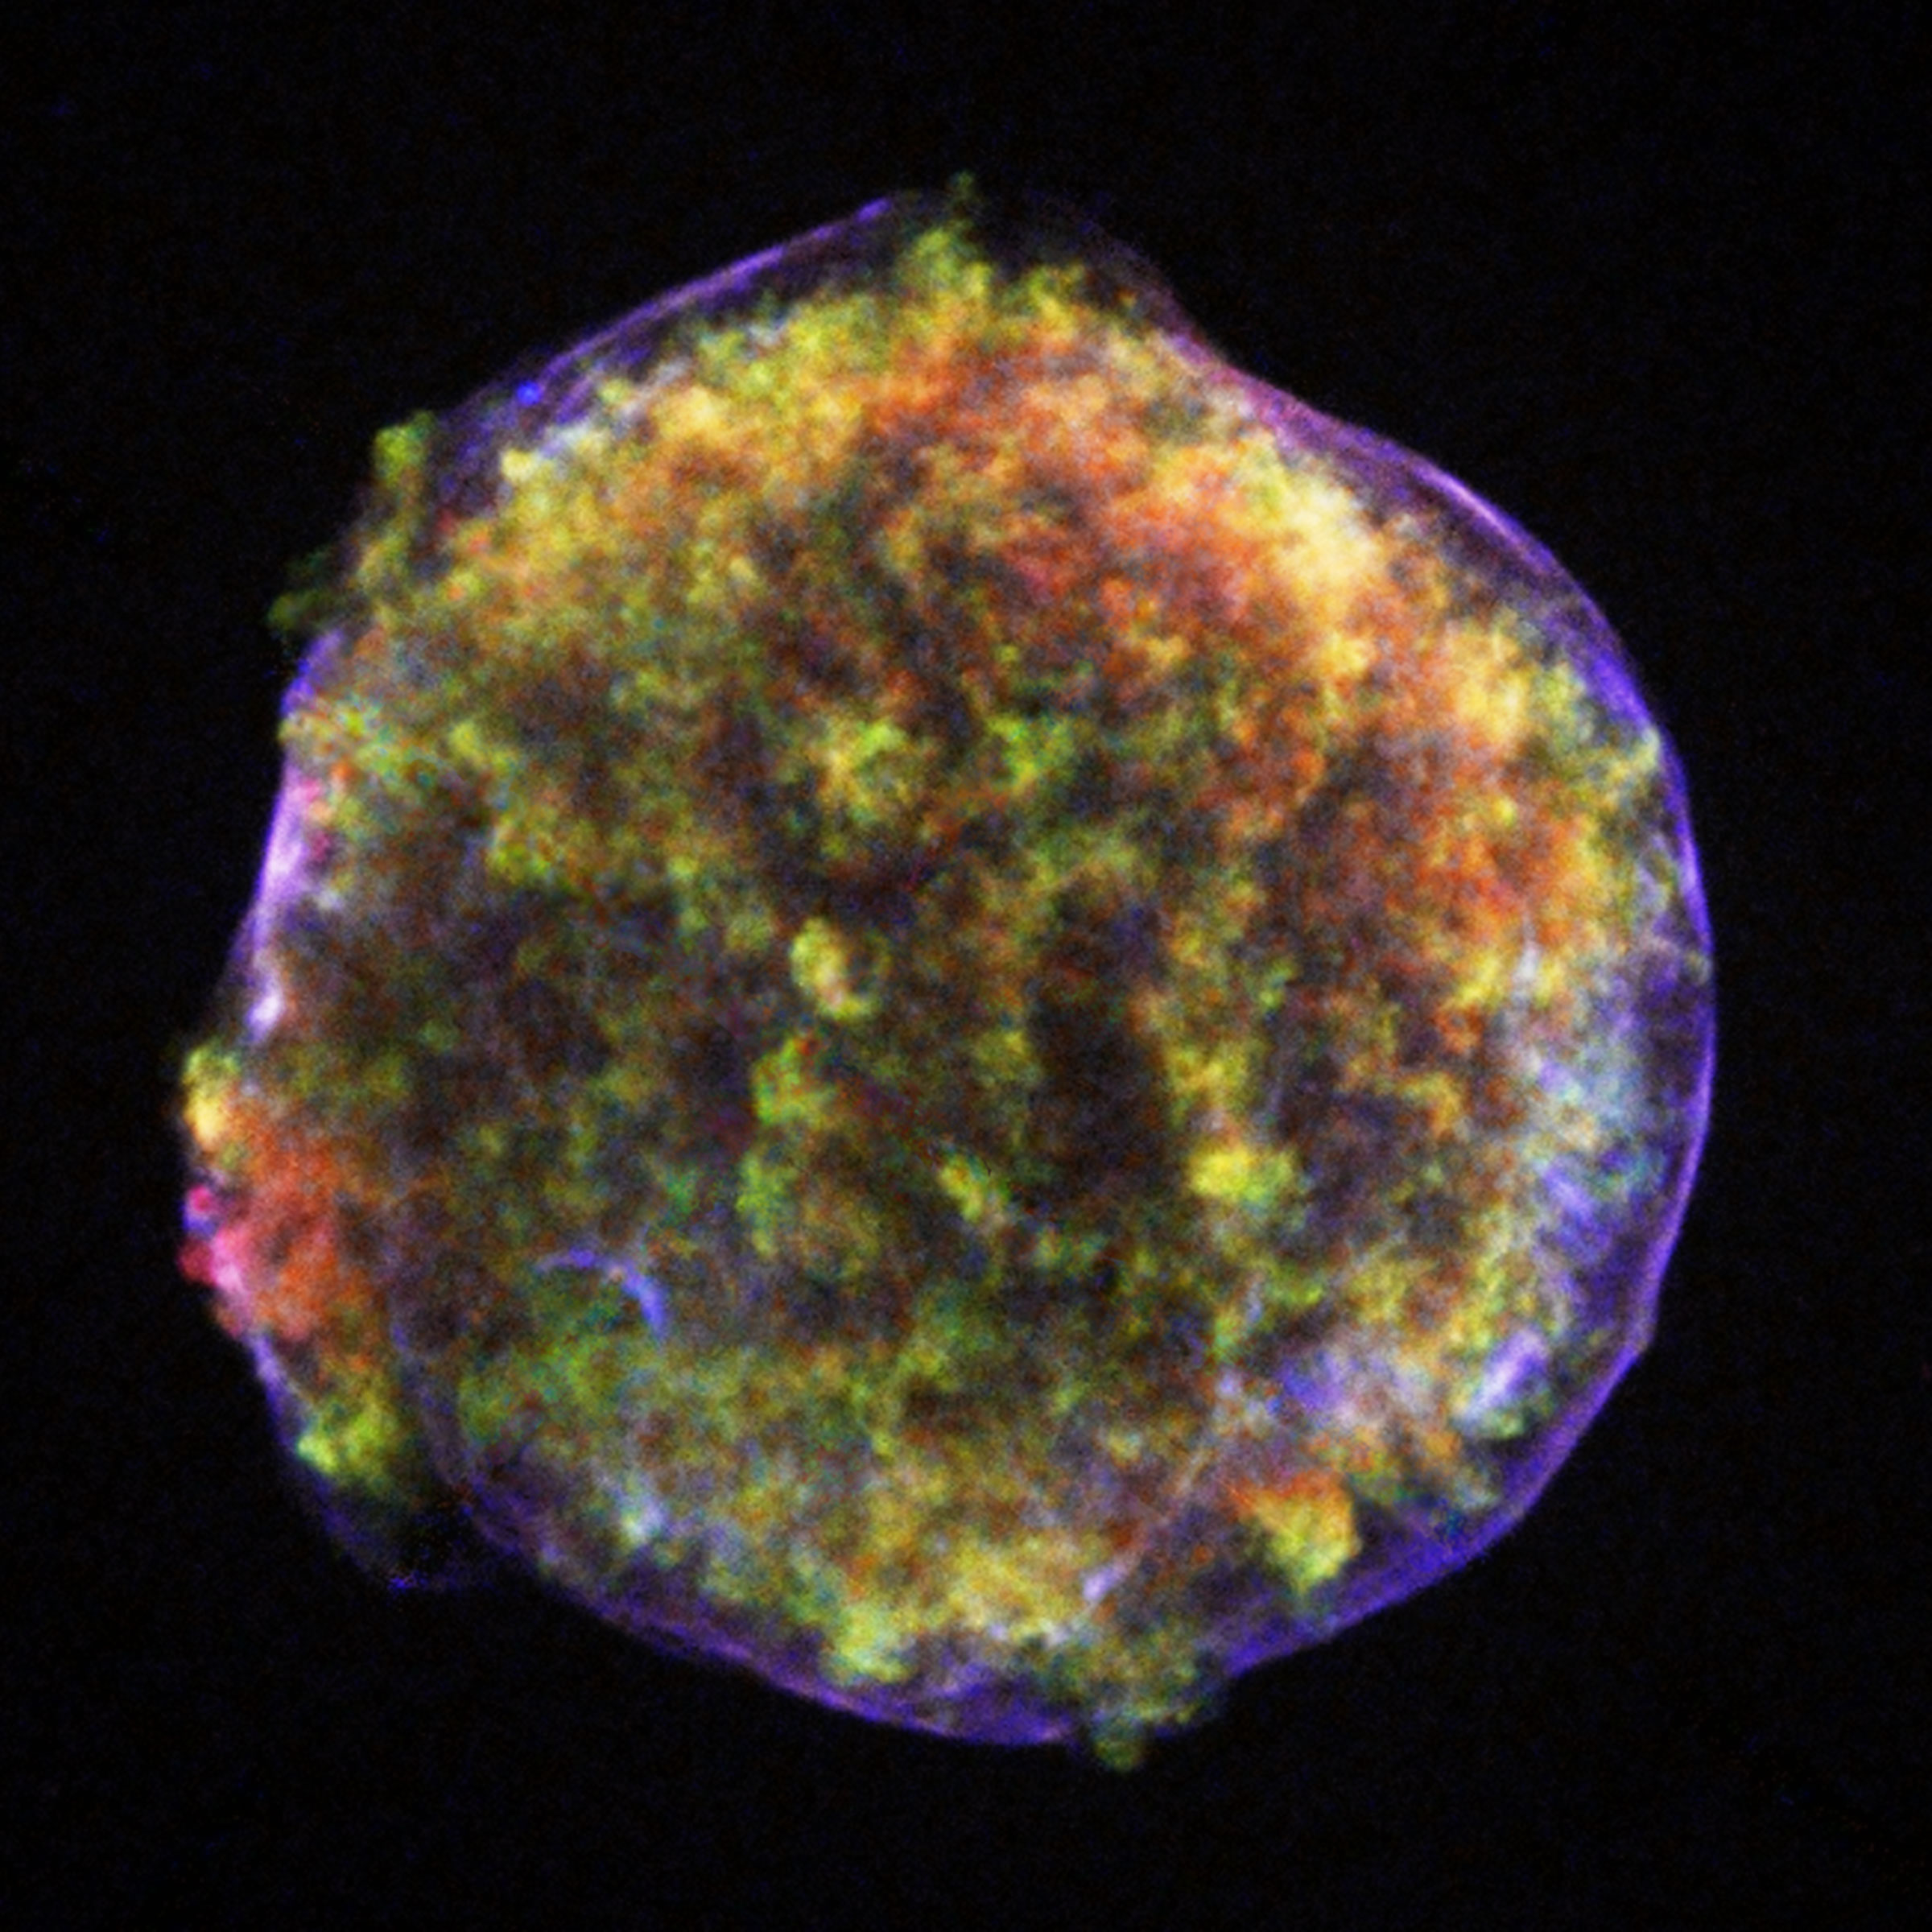
\includegraphics[width=\columnwidth]{images/Tycho-Supernova.jpg}\caption{X-ray image of SN\,1572, Chandra X-ray Observatory.}\end{figure}}
\vs p041 3:6 \pc Not all stars are solid, but many of the older ones are. Some of the reddish, faintly glimmering stars have acquired a density at the centre of their enormous masses which would be expressed by saying that 1 cm\ts{3} of such a star, if on Urantia, would weigh 166\,kg. The enormous pressure, accompanied by loss of heat and circulating energy, has resulted in bringing the orbits of the basic material units closer and closer together until they now closely approach the status of electronic condensation. This process of cooling and contraction may continue to the limiting and critical explosion point of ultimatonic condensation.
\vs p041 3:7 Most of the giant suns are relatively young; most of the dwarf stars are old, but not all. The collisional dwarfs may be very young and may glow with an intense white light, never having known an initial red stage of youthful shining. Both very young and very old suns usually shine with a reddish glow. The yellow tinge indicates moderate youth or approaching old age, but the brilliant white light signifies robust and extended adult life.
\vs p041 3:8 \pc While all adolescent suns do not pass through a pulsating stage, at least not visibly, when looking out into space you may observe many of these younger stars whose gigantic respiratory heaves require from 2 to 7 days to complete a cycle. Your own sun still carries a diminishing legacy of the mighty upswellings of its younger days, but the period has lengthened from the former 3½ day pulsations to the present 11½ year sunspot cycles.
\vs p041 3:9 Stellar variables have numerous origins. In some double stars the tides caused by rapidly changing distances as the two bodies swing around their orbits also occasion periodic fluctuations of light. These gravity variations produce regular and recurrent flares, just as the capture of meteors by the accretion of energy\hyp{}material at the surface would result in a comparatively sudden flash of light which would speedily recede to normal brightness for that sun. Sometimes a sun will capture a stream of meteors in a line of lessened gravity opposition, and occasionally collisions cause stellar flare\hyp{}ups, but the majority of such phenomena are wholly due to internal fluctuations.
\vs p041 3:10 In one group of variable stars the period of light fluctuation is directly dependent on luminosity, and knowledge of this fact enables astronomers to utilize such suns as universe lighthouses or accurate measuring points for the further exploration of distant star clusters. By this technique it is possible to measure stellar distances most precisely up to more than 1,000,000 light\hyp{}years. Better methods of space measurement and improved telescopic technique will sometime more fully disclose the 10 grand divisions of the superuniverse of Orvonton; you will at least recognize 8 of these immense sectors as enormous and fairly symmetrical star clusters.
\usection{Sun Density}
\vs p041 4:1 The mass of your sun is slightly greater than the estimate of your physicists, who have reckoned it as about $2\times 10^{30}$\,kg\fnst{The present estimate is: $1.98892 \times 10^{30}$ kg.}. It now exists about halfway between the most dense and the most diffuse stars, having about 1.5 times the density of water\fnst{More accurately: $1.408 \times 10^3$\,kg/m\ts{3}.}. But your sun is neither a liquid nor a solid --- it is gaseous --- and this is true notwithstanding the difficulty of explaining how gaseous matter can attain this and even much greater densities.
\vs p041 4:2 \pc Gaseous, liquid, and solid states are matters of atomic\hyp{}molecular relationships, but density is a relationship of space and mass. Density varies directly with the quantity of mass in space and inversely with the amount of space in mass, the space between the central cores of matter and the particles which whirl around these centres as well as the space within such material particles.
\vs p041 4:3 \pc Cooling stars can be physically gaseous and tremendously dense at the same time. You are not familiar with the solar \bibemph{supergases,}\fnst{In the original source text \cite{Eddington1} the phrase ``not imperfect, but superperfect'' explains the prefix ``super''.} but these and other unusual forms of matter explain how even nonsolid suns can attain a density equal to iron --- about the same as Urantia --- and yet be in a highly heated gaseous state and continue to function as suns. The atoms in these dense supergases are exceptionally small; they contain few electrons. Such suns have also largely lost their free ultimatonic stores of energy.
\vs p041 4:4 One of your near\hyp{}by suns, which started life with about the same mass as yours, has now contracted almost to the size of Urantia, having become 40,000\fnst{In 1955 text ``sixty thousand''. Textual consistency and current scientific estimates of our sun’s density both support the change to “40,000.” The first paragraph of this section states that our sun is about 1.5 times the density of water 1 g/cm\ts{3}, and 40,000 times this is 40 kg/cm\ts{3}; the current scientific estimate of the sun’s density is 1.4 times the density of water; 40,000 times that is 56 kg/cm\ts{3}. The likely cause of this error in the 1955 text is that the number in question was written as a numeral in the manuscript (40,000 not forty thousand), and the error was caused by a simple keystroke error in which 6 was mis-keyed for 4, creating 60,000 instead of 40,000. When the text was formatted for printing, the numerals were changed to words, and an error that formerly consisted of one digit was transformed into an incorrect word. The formatting of words and numbers for printing is not a revelatory issue; it is a matter of style, and is covered extensively in the Chicago Manual of Style. (The problem at \bibref[43:1.6]{p043 1:6} in the text appears to have had an identical origin, and \bibref[42:5.1]{p042 5:1} in the text is very closely related.)} times as dense as your sun. The weight of this hot\hyp{}cold gaseous\hyp{}solid is about 61 kg/cm\ts{3}\fnst{Calculating the density we obtain $\rho = 1851.8$\,kg/cm\ts{3}, which differs greatly from the figure 61\,kg/cm\ts{3} given in the text. Therefore, this ``near-by sun'' has lost most of its mass by now.}. And still this sun shines with a faint reddish glow, the senile glimmer of a dying monarch of light.
\vs p041 4:5 Most of the suns, however, are not so dense. One of your nearer neighbours\fnst{The distance to Capella (α Aurig\ae) is estimated to be about 43 light years.} has a density exactly equal to that of your atmosphere at sea level. If you were in the interior of this sun, you would be unable to discern anything. And temperature permitting, you could penetrate the majority of the suns which twinkle in the night sky and notice no more matter than you perceive in the air of your earthly living rooms.
\vs p041 4:6 The massive sun of Veluntia, one of the largest in Orvonton, has a density only 0.001 that of Urantia’s atmosphere. Were it in composition similar to your atmosphere and not superheated, it would be such a vacuum that human beings would speedily suffocate if they were in or on it.
\vs p041 4:7 Another of the Orvonton giants now has a surface temperature a trifle under 3,000\,°C. Its diameter is over 482,803,200\,km --- ample room to accommodate your sun and the present orbit of the earth. And yet, for all this enormous size, over 40,000,000 times\fnst{Here the ``size'' obviously signifies the volume, not the diameter, because the diameter of the Sun is 1,391,400\,km and therefore the ratio of volumes of the two stars is 41,778,652, i.e. approximately 40,000,000.} that of your sun, its mass is only about 30 times greater. These enormous suns have an extending fringe that reaches almost from one to the other.
\usection{Solar Radiation}
\vs p041 5:1 That the suns of space are not very dense is proved by the steady streams of escaping light\hyp{}energies. Too great a density would retain light by opacity until the light\hyp{}energy pressure reached the explosion point. There is a tremendous light or gas pressure within a sun to cause it to shoot forth such a stream of energy as to penetrate space for millions upon millions of kilometres to energize, light, and heat the distant planets. 4.6\,m of surface of the density of Urantia would effectually prevent the escape of all X\hyp{}rays and light\hyp{}energies from a sun until the rising internal pressure of accumulating energies resulting from atomic dismemberment overcame gravity with a tremendous outward explosion.
\vs p041 5:2 Light, in the presence of the propulsive gases, is highly explosive when confined at high temperatures by opaque retaining walls. Light is real. As you value energy and power on your world, sunlight would be economical at a million pounds sterling a kilogram.
\vs p041 5:3 The interior of your sun is a vast X\hyp{}ray generator. The suns are supported from within by the incessant bombardment of these mighty emanations.
\vs p041 5:4 It requires more than 500,000 years for an X\hyp{}ray\hyp{}stimulated electron to work its way from the very centre of an average sun up to the solar surface, whence it starts out on its space adventure, maybe to warm an inhabited planet, to be captured by a meteor, to participate in the birth of an atom, to be attracted by a highly charged dark island of space, or to find its space flight terminated by a final plunge into the surface of a sun similar to the one of its origin.
\vs p041 5:5 The X\hyp{}rays of a sun’s interior charge the highly heated and agitated electrons with sufficient energy to carry them out through space, past the hosts of detaining influences of intervening matter and, in spite of divergent gravity attractions, on to the distant spheres of the remote systems. The great energy of velocity required to escape the gravity clutch of a sun is sufficient to ensure that the sunbeam will travel on with unabated velocity until it encounters considerable masses of matter; whereupon it is quickly transformed into heat with the liberation of other energies.
\vs p041 5:6 \pc Energy, whether as light or in other forms, in its flight through space moves straight forward. The actual particles of material existence traverse space like a fusillade. They go in a straight and unbroken line or procession except as they are acted on by superior forces, and except as they ever obey the linear\hyp{}gravity pull inherent in material mass and the circular\hyp{}gravity presence of the Isle of Paradise.
\vs p041 5:7 \pc Solar energy may seem to be propelled in waves, but that is due to the action of coexistent and diverse influences. A given form of organized energy does not proceed in waves but in direct lines. The presence of a second or a third form of force\hyp{}energy may cause the stream under observation to \bibemph{appear} to travel in wavy formation, just as, in a blinding rainstorm accompanied by a heavy wind, the water sometimes appears to fall in sheets or to descend in waves. The raindrops are coming down in a direct line of unbroken procession, but the action of the wind is such as to give the visible appearance of sheets of water and waves of raindrops.
\vs p041 5:8 The action of certain secondary and other undiscovered energies present in the space regions of your local universe is such that solar\hyp{}light emanations appear to execute certain wavy phenomena as well as to be chopped up into infinitesimal portions of definite length and weight. And, practically considered, that is exactly what happens. You can hardly hope to arrive at a better understanding of the behaviour of light until such a time as you acquire a clearer concept of the interaction and interrelationship of the various space\hyp{}forces and solar energies operating in the space regions of Nebadon. Your present confusion is also due to your incomplete grasp of this problem as it involves the interassociated activities of the personal and nonpersonal control of the master universe --- the presences, the performances, and the co\hyp{}ordination of the Conjoint Actor and the Unqualified Absolute.
\usection{Calcium --- The Wanderer of Space}
\vs p041 6:1 In deciphering spectral phenomena, it should be remembered that space is not empty; that light, in traversing space, is sometimes slightly modified by the various forms of energy and matter which circulate in all organized space. Some of the lines indicating unknown matter which appear in the spectra of your sun are due to modifications of well\hyp{}known elements which are floating throughout space in shattered form, the atomic casualties of the fierce encounters of the solar elemental battles. Space is pervaded by these wandering derelicts, especially sodium and calcium.
\vs p041 6:2 Calcium is, in fact, the chief element of the matter\hyp{}permeation of space throughout Orvonton. Our whole superuniverse is sprinkled with minutely pulverized stone. Stone is literally the basic building matter for the planets and spheres of space. The cosmic cloud, the great space blanket, consists for the most part of the modified atoms of calcium. The stone atom is one of the most prevalent and persistent of the elements. It not only endures solar ionization --- splitting --- but persists in an associative identity even after it has been battered by the destructive X\hyp{}rays and shattered by the high solar temperatures. Calcium possesses an individuality and a longevity excelling all of the more common forms of matter.
\vs p041 6:3 \pc As your physicists have suspected, these mutilated remnants of solar calcium literally ride the light beams for varied distances, and thus their widespread dissemination throughout space is tremendously facilitated. The sodium atom, under certain modifications, is also capable of light and energy locomotion. The calcium feat is all the more remarkable since this element has almost twice the mass of sodium. Local space\hyp{}permeation by calcium is due to the fact that it escapes from the solar photosphere, in modified form, by literally riding the outgoing sunbeams. Of all the solar elements, calcium, notwithstanding its comparative bulk --- containing as it does 20 revolving electrons --- is the most successful in escaping from the solar interior to the realms of space. This explains why there is a calcium layer, a gaseous stone surface, on the sun 9,600\,km thick; and this despite the fact that 19 lighter elements, and numerous heavier ones, are underneath.
\vs p041 6:4 Calcium is an active and versatile element at solar temperatures. The stone atom has two agile and loosely attached electrons in the two outer electronic circuits, which are very close together. Early in the atomic struggle it loses its outer electron; whereupon it engages in a masterful act of juggling the 19\ts{th} electron back and forth between the 19\ts{th} and 20\ts{th} circuits of electronic revolution. By tossing this 19\ts{th} electron back and forth between its own orbit and that of its lost companion more than 25,000 times a second, a mutilated stone atom is able partially to defy gravity and thus successfully to ride the emerging streams of light and energy, the sunbeams, to liberty and adventure. This calcium atom moves outward by alternate jerks of forward propulsion, grasping and letting go the sunbeam about 25,000 times each second. And this is why stone is the chief component of the worlds of space. Calcium is the most expert solar\hyp{}prison escaper.
\vs p041 6:5 The agility of this acrobatic calcium electron is indicated by the fact that, when tossed by the temperature\hyp{}X\hyp{}ray solar forces to the circle of the higher orbit, it only remains in that orbit for about $10^{-6}$ seconds; but before the electric\hyp{}gravity power of the atomic nucleus pulls it back into its old orbit, it is able to complete 1,000,000 revolutions about the atomic centre.
\vs p041 6:6 \pc Your sun has parted with an enormous quantity of its calcium, having lost tremendous amounts during the times of its convulsive eruptions in connection with the formation of the solar system. Much of the solar calcium is now in the outer crust of the sun.
\vs p041 6:7 \pc It should be remembered that spectral analyses show only sun\hyp{}surface compositions. For example: Solar spectra exhibit many iron lines, but iron is not the chief element in the sun. This phenomenon is almost wholly due to the present temperature of the sun’s surface, a little less than 6,000\,°C, this temperature being very favourable to the registry of the iron spectrum.
\usection{Sources of Solar Energy}
\vs p041 7:1 The internal temperature of many of the suns, even your own, is much higher than is commonly believed. In the interior of a sun practically no whole atoms exist; they are all more or less shattered by the intensive X\hyp{}ray bombardment which is indigenous to such high temperatures. Regardless of what material elements may appear in the outer layers of a sun, those in the interior are rendered very similar by the dissociative action of the disruptive X\hyp{}rays. X\hyp{}ray is the great leveler of atomic existence.
\vs p041 7:2 The surface temperature of your sun is almost 6,000\,°C\fnst{The American text of 1955 says ``6,000 degrees'' and specifies that it refers to ``your Fahrenheit scale''. However, the number 6,000 is clearly taken from p.\,14 of \cite{Eddington1}, where it refers to our Centigrade (Celsius) scale, as is indicated in the Preface on p.~6 of this work. Therefore, the modern estimates of the temperature of our Sun's photosphere (5,778\,K) are in agreement with the value given in this Revelation, as long as the units discrepancy is taken into count. What happened here is that Dr~Sadler quoted the text of \cite{Eddington1}, but forgot about the warning given concerning the units in the Preface thereof. Exactly the same situation occurred with the ``English vs American billions'' issue below, see \bibref[41:9.3]{p041 9:3}.}, but it rapidly increases as the interior is penetrated until it attains the unbelievable height of about 35,000,000\,°C in the central regions. (All of these temperatures refer to your Celsius\fnst{In 1955 text ``Fahrenheit''. However, it is now perfectly clear that these temperatures were taken from Eddington's book ``Stars and Atoms'' \cite{Eddington1} without converting the units from Celsius to Fahrenheit.} scale.)
\vs p041 7:3 \pc All of these phenomena are indicative of enormous energy expenditure, and the sources of solar energy, named in the order of their importance, are:
\vs p041 7:4 \ublistelem{1.}\bibnobreakspace Annihilation of atoms and, eventually, of electrons.
\vs p041 7:5 \ublistelem{2.}\bibnobreakspace Transmutation of elements, including the radioactive group of energies thus liberated.
\vs p041 7:6 \ublistelem{3.}\bibnobreakspace The accumulation and transmission of certain universal space\hyp{}energies.
\vs p041 7:7 \ublistelem{4.}\bibnobreakspace Space matter and meteors which are incessantly diving into the blazing suns.
\vs p041 7:8 \ublistelem{5.}\bibnobreakspace Solar contraction; the cooling and consequent contraction of a sun yields energy and heat sometimes greater than that supplied by space matter.
\vs p041 7:9 \ublistelem{6.}\bibnobreakspace Gravity action at high temperatures transforms certain circuitized power into radiative energies.
\vs p041 7:10 \ublistelem{7.}\bibnobreakspace Recaptive light and other matter which are drawn back into the sun after having left it, together with other energies having extrasolar origin.
\vs p041 7:11 \pc There exists a regulating blanket of hot gases (sometimes millions of degrees in temperature) which envelops the suns, and which acts to stabilize heat loss and otherwise prevent hazardous fluctuations of heat dissipation. During the active life of a sun the internal temperature of 35,000,000\,°C remains about the same quite regardless of the progressive fall of the external temperature.
\vs p041 7:12 \pc You might try to visualize 35,000,000\,°C of heat, in association with certain gravity pressures, as the electronic boiling point\fnst{The upper bound for the electronic boiling point was calculated on the basis of the general relativistic covariant nonlocal statistical dynamics to be 740,000,000\,K at by A.A.~Vlasov in \cite{Vlasov1} and the actual value estimated by comparison with the energy distribution of cosmic rays at 657,000,000\,K. This was done without taking into account the quantum effects. The corresponding quantum calculation has not yet been done by anyone.}. Under such pressure and at such temperature all atoms are degraded and broken up into their electronic and other ancestral components; even the electrons and other associations of ultimatons may be broken up, but the suns are not able to degrade the ultimatons.
\vs p041 7:13 These solar temperatures operate to enormously speed up the ultimatons and the electrons, at least such of the latter as continue to maintain their existence under these conditions. You will realize what high temperature means by way of the acceleration of ultimatonic and electronic activities when you pause to consider that one drop of ordinary water contains over $10^{21}$ of atoms\fnst{The mass of such a drop would be: $m = 1/3\times(2 m_H + m_O)\times 10^{21} = 0.01\,g$.}. This is the energy of more than 100 horsepower exerted continuously for two years\fnst{Assuming the value of 1\,horsepower = 745.7\,watts, we obtain for the energy $E = 100\times 745.7\times 2\times 365\times 86,400 = 4.7\times 10^{12}\,J$. Using Einstein's formula $E = mc^2$, we can calculate the mass of the drop: $m = E/c^2 = 0.05\,g$. This is five times greater than the estimate obtained in the previous note, based on the number of atoms in the drop. Therefore, either Einstein's formula is incorrect (but then how to reconcile this with the statement made in \bibref[42:4.11]{p042 4:11}?) or the masses of hydrogen and oxygen atoms are different from the present values or, perhaps, the revelators are not overly concerned with being absolutely accurate in such minor technical details. It is, however, curious that this example is taken from pp.\,102--103 of \cite{Eddington1}, where the author commits the same mistake, which is carried over here.}. The total heat now given out by the solar system sun each second is sufficient to boil all the water in all the oceans on Urantia in just one second of time.
\vs p041 7:14 \pc Only those suns which function in the direct channels of the main streams of universe energy can shine on forever. Such solar furnaces blaze on indefinitely, being able to replenish their material losses by the intake of space\hyp{}force and analogous circulating energy. But stars far removed from these chief channels of recharging are destined to undergo energy depletion --- gradually cool off and eventually burn out.
\vs p041 7:15 Such dead or dying suns can be rejuvenated by collisional impact or can be recharged by certain nonluminous energy islands of space or through gravity\hyp{}robbery of near\hyp{}by smaller suns or systems. The majority of dead suns will experience revivification by these or other evolutionary techniques. Those which are not thus eventually recharged are destined to undergo disruption by mass explosion when the gravity condensation attains the critical level of ultimatonic condensation of energy pressure. Such disappearing suns thus become energy of the rarest form, admirably adapted to energize other more favourably situated suns.
\usection{Solar\hyp{}Energy Reactions}
\vs p041 8:1 In those suns which are encircuited in the space\hyp{}energy channels, solar energy is liberated by various complex nuclear\hyp{}reaction chains, the most common of which is the hydrogen\hyp{}carbon\hyp{}helium reaction. In this metamorphosis, carbon acts as an energy catalyst since it is in no way actually changed by this process of converting hydrogen into helium. Under certain conditions of high temperature the hydrogen penetrates the carbon nuclei. Since the carbon cannot hold more than four such protons, when this saturation state is attained, it begins to emit protons as fast as new ones arrive. In this reaction the ingoing hydrogen particles come forth as a helium atom.
\vs p041 8:2 \pc Reduction of hydrogen content increases the luminosity of a sun. In the suns destined to burn out, the height of luminosity is attained at the point of hydrogen exhaustion. Subsequent to this point, brilliance is maintained by the resultant process of gravity contraction. Eventually, such a star will become a so\hyp{}called white dwarf, a highly condensed sphere.
\vs p041 8:3 \pc In large suns --- small circular nebulae --- when hydrogen is exhausted and gravity contraction ensues, if such a body is not sufficiently opaque to retain the internal pressure of support for the outer gas regions, then a sudden collapse occurs. The gravity\hyp{}electric changes give origin to vast quantities of tiny particles devoid of electric potential, and such particles readily escape from the solar interior, thus bringing about the collapse of a gigantic sun within a few days. It was such an emigration of these “runaway particles” that occasioned the collapse of the giant nova of the Andromeda nebula about 50 years ago. This vast stellar body collapsed in 40 minutes of Urantia time.
\vs p041 8:4 As a rule, the vast extrusion of matter continues to exist about the residual cooling sun as extensive clouds of nebular gases. And all this explains the origin of many types of irregular nebulae, such as the Crab nebula, which had its origin about 900 years ago, and which still exhibits the mother sphere as a lone star near the centre of this irregular nebular mass.\tunemarkup{pictures}{\begin{figure}[H]\centering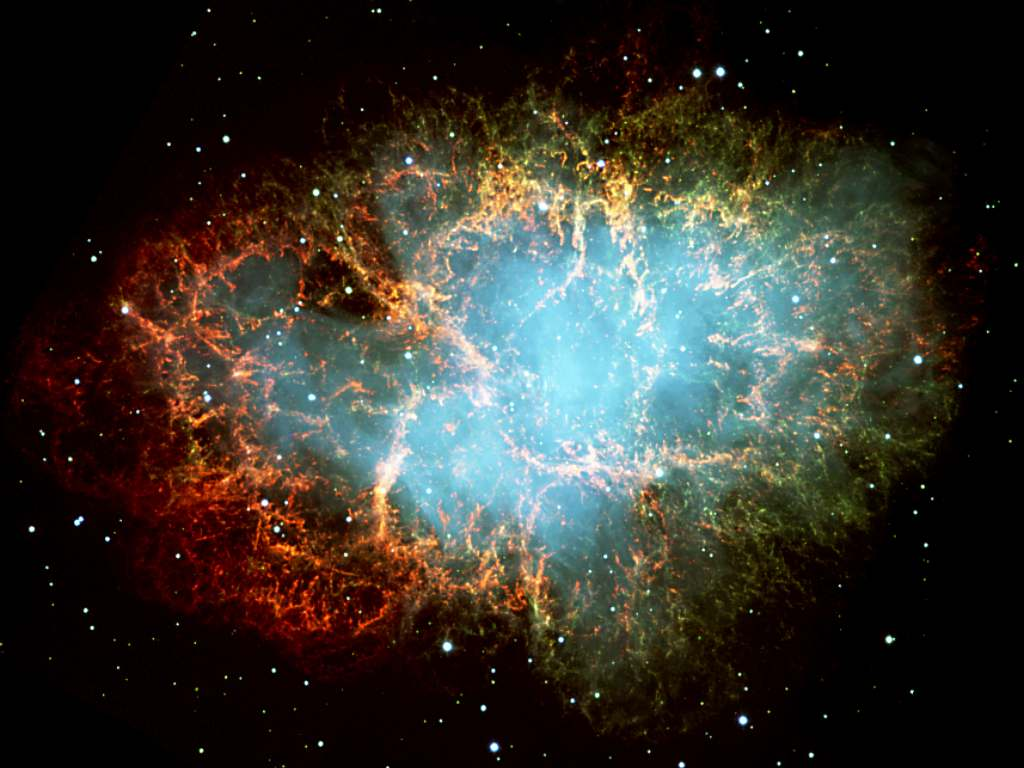
\includegraphics[width=\columnwidth]{images/crab.jpg}\caption{The Crab Nebula from VLT}\end{figure}}
\usection{Sun Stability}
\vs p041 9:1 The larger suns maintain such a gravity control over their electrons that light escapes only with the aid of the powerful X\hyp{}rays. These helper rays penetrate all space and are concerned in the maintenance of the basic ultimatonic associations of energy. The great energy losses in the early days of a sun, subsequent to its attainment of maximum temperature --- upwards of 35,000,000\,°C --- are not so much due to light escape as to ultimatonic leakage. These ultimaton energies escape out into space, to engage in the adventure of electronic association and energy materialization, as a veritable energy blast during adolescent solar times.
\vs p041 9:2 \pc Atoms and electrons are subject to gravity. The ultimatons are \bibemph{not} subject to local gravity, the interplay of material attraction, but they are fully obedient to absolute or Paradise gravity, to the trend, the swing, of the universal and eternal circle of the universe of universes. Ultimatonic energy does not obey the linear or direct gravity attraction of near\hyp{}by or remote material masses, but it does ever swing true to the circuit of the great ellipse of the far\hyp{}flung creation.
\vs p041 9:3 \pc Your own solar centre radiates almost $10^{14}$\fnst{The American text of 1955 says ``one hundred billion'', but this is a quotation from p.98 of \cite{Eddington1}, where the \bibemph{English} billions (million million) are used and not the \bibemph{American} billions, i.e. thousand million. Otherwise, the figure given in the text would be thousand times smaller than the actual value well-known in the modern science. The author, Sir Arthur S.~Eddington explicitly warns the American reader in the Preface, but, apparently, Dr~Sadler did not notice this warning.} tons of actual matter annually, while the giant suns lose matter at a prodigious rate during their earlier growth, the first billion years. A sun’s life becomes stable after the maximum of internal temperature is reached, and the subatomic energies begin to be released. And it is just at this critical point that the larger suns are given to convulsive pulsations.
\vs p041 9:4 Sun stability is wholly dependent on the equilibrium between gravity\hyp{}heat contention --- tremendous pressures counterbalanced by unimagined temperatures. The interior gas elasticity of the suns upholds the overlying layers of varied materials, and when gravity and heat are in equilibrium, the weight of the outer materials exactly equals the temperature pressure of the underlying and interior gases. In many of the younger stars continued gravity condensation produces ever\hyp{}heightening internal temperatures, and as internal heat increases, the interior X\hyp{}ray pressure of supergas winds becomes so great that, in connection with the centrifugal motion, a sun begins to throw its exterior layers off into space, thus redressing the imbalance between gravity and heat.
\vs p041 9:5 Your own sun has long since attained relative equilibrium between its expansion and contraction cycles, those disturbances which produce the gigantic pulsations of many of the younger stars. Your sun is now passing out of its six billionth year. At the present time it is functioning through the period of greatest economy. It will shine on as of present efficiency for more than $2.5 \times 10^{10}$ years. It will probably experience a partially efficient period of decline as long as the combined periods of its youth and stabilized function.
\usection{Origin of Inhabited Worlds}
\vs p041 10:1 Some of the variable stars, in or near the state of maximum pulsation, are in process of giving origin to subsidiary systems, many of which will eventually be much like your own sun and its revolving planets. Your sun was in just such a state of mighty pulsation when the massive Angona system swung into near approach, and the outer surface of the sun began to erupt veritable streams --- continuous sheets --- of matter. This kept up with ever\hyp{}increasing violence until nearest apposition, when the limits of solar cohesion were reached and a vast pinnacle of matter, the ancestor of the solar system, was disgorged. In similar circumstances the closest approach of the attracting body sometimes draws off whole planets, even a \bibfrac{1}{4}\ts{th} or \bibfrac{1}{3}\ts{rd} of a sun. These major extrusions form certain peculiar cloud\hyp{}bound types of worlds, spheres much like Jupiter\index{Planets!Jupiter} and Saturn\index{Planets!Saturn}.
\vs p041 10:2 The majority of solar systems, however, had an origin entirely different from yours, and this is true even of those which were produced by gravity\hyp{}tidal technique. But no matter what technique of world building obtains, gravity always produces the solar system type of creation; that is, a central sun or dark island with planets, satellites, subsatellites, and meteors.
\vs p041 10:3 \pc The physical aspects of the individual worlds are largely determined by mode of origin, astronomical situation, and physical environment. Age, size, rate of revolution, and velocity through space are also determining factors. Both the gas\hyp{}contraction and the solid\hyp{}accretion worlds are characterized by mountains and, during their earlier life, when not too small, by water and air. The molten\hyp{}split and collisional worlds are sometimes without extensive mountain ranges.
\vs p041 10:4 During the earlier ages of all these new worlds, earthquakes are frequent, and they are all characterized by great physical disturbances; especially is this true of the gas\hyp{}contraction spheres, the worlds born of the immense nebular rings which are left behind in the wake of the early condensation and contraction of certain individual suns. Planets having a dual origin like Urantia pass through a less violent and stormy youthful career. Even so, your world experienced an early phase of mighty upheavals, characterized by volcanoes, earthquakes, floods, and terrific storms.
\vs p041 10:5 \pc Urantia is comparatively isolated on the outskirts of Satania, your solar system, with one exception, being the farthest removed from Jerusem, while Satania itself is next to the outermost system of Norlatiadek, and this constellation is now traversing the outer fringe of Nebadon. You were truly among the least of all creation until Michael’s bestowal elevated your planet to a position of honour and great universe interest. Sometimes the last is first, while truly the least becomes greatest.
\vsetoff
\vs p041 10:6 [Presented by an Archangel in collaboration with the Chief of Nebadon Power Centres.]
\quizlink
\begin{thebibliography}{100}
\bibitem{Eddington1}
A.S.~Eddington
{``Stars and Atoms''}
{\em Oxford: Clarendon Press}, 1927.
\bibitem{Jeans1}
J.~Jeans.
{``Through Space and Time''}
{\em Cambridge: University Press}, 1934.
\bibitem{Vlasov1}
A.A.~Vlasov.
{``Nonlocal Statistical Mechanics'' (in Russian)}
{\em Moscow}, 1978.
\end{thebibliography}
